\section{M-SPLearning}\label{section3}

%Com o objetivo de apresentar como o gerenciamento da variabilidades pode melhorar o desenvolvimento de aplicações de m-learning, os autores definiram uma LPS, denominada M-SPLearning. Buscando explorar as variabilidades desse domínio para acelerar o time to market e reduzir o numero de falhas nos produtos. Nesta seção, as atividades conduzidas para a concepção da M-SPLearning são detalhadas a fim de expor suas principais peculiaridades e referências.
Aiming at presenting how the management of variabilities can improve the development of m-learning applications, we have established M-SPLearning \cite{falvojr14a, falvojr14b}. The idea is to investigate how the variabilities of this domain can accelerate time-to-market and reduce product faults. In this section, the activities conducted in design of the M-SPLearning are detailed \cite{oliveirajr10, filho13, krueger02, kang90}.

%A Seção \ref{section31} apresenta a Engenharia de Domínio realizada para concepção da \textit{M-SPLear\allowbreak ning} evidenciando sua capacidade produtiva através das seguintes atividades secundárias: (i) Análise de Domínio; (ii) Definição da Arquitetura; (iii) Projeto de Componentes; e (iv) Plano de Produção. Em seguida, na Seção \ref{section32}, a Engenharia de Aplicação apresenta os detalhes sobre a implementação e utilização da LPS especificada.
%Section \ref{section31} presents the DE performed for the M-SPLearning design showing its productive capacity by means of the following sideline activities: (i) Domain Analysis; (ii) Definition of Architecture; (iii) Components Design; and (iv) Production Plan. In Section \ref{section32}, AE details the implementation and utilization of our SPL.

\subsection{Domain Engineering}\label{section31}

%Durante a atividade de Engenharia Domínio as similaridades e variabilidades devem ser eliciadas para o desenvolvimento de LPS, a fim de estabelecer uma plataforma reutilizável sistemática. O resultado desta atividade é um conjunto de ativos com os quais a LPS deve ser implementada, caracterizando, assim, sua família de produtos. Em geral, as actividades que caracterizam a Engenharia de Domínio pode ser consideradas as mais críticas durante a concepção de uma LPS, dado que delimitar um domínio de estudo não é uma tarefa trivial.
During the DE activity, similarities and variabilities must be specified for the development of the SPL in order to establish a systematic reusable platform. The result of this activity is a set of assets from which the SPL should be implemented, thus characterizing its product family \cite{bockle05, vanderlinden07}. In general, the activities that characterize the DE can be considered the most critical in the conception of an SPL, since delimiting a domain of study is not a trivial task.

%Analisando o extenso domínio das aplicações móveis percebe-se que seus produtos podem ser implementadas usando diferentes plataformas de desenvolvimento, como por exemplo, Android, iOS ou Windows Phone. Com isto, o domínio de m-learning também inclui sistemas operacionais diferentes. Assim, para definir um domínio aceitável em termos de escopo, selecionamos um único sistema operacional. Nossa escolha pelo Android se baseou na quantidade de dispositivos que cada sistema operacional controla, visto que esse SO detém cerca de 80% do mercado de smartphones do mundo, equivalente a 793,6 milhões de dispositivos.
Mobile applications can be implemented using different development platforms, including Android, iOS and Windows Phone. Furthermore, the m-learning domain also includes different operating systems. Thus, to define an acceptable domain in terms of scope, we selected a single operating system. Our choice for Android was based on the amount of devices that each operating system controls, since this OS owns around 80\% of the world's smartphones market, which is equivalent to 793.6 million devices. \cite{llamas14}.

%Com um domínio factível definido, um catálogo de requisitos para ambientes m-learning foi adaptado respeitando o modelo de qualidade ISO/IEC 25010, gerando, assim, um catálogo de requisitos estendido e, em seguida, o modelo de features para a M-SPLearning. Tal catálogo busca refletir, em alto nível, a experiência adquirida pelos desenvolvedores e pesquisadores nesta nova modalidade de aprendizagem. Além disso, o catálogo é genérico e abrangente, beneficiando sua adoção para fins diferentes do domínio de m-learning.
With a feasible domain defined, a requirements catalog for m-learning applications was proposed based on a related work \cite{filho13} and ISO/IEC 25010 quality model. Such a catalog intends to reflect, in a high level basis, the experience gained from developers and researchers of m-learning. Furthermore, the catalog is generic and embracing, benefiting its adoption for different purposes in the m-learning domain. 

%Para o gerenciamento das variabilidades em questão a M-SPLearning foi desenvolvida com base na abordagem SMarty. Entre as razões para a nossa escolha, destacam-se: (i) a facilidade cognitiva fornecida pela SMarty, apoiada por várias ferramentas de modelagem; (ii) a sua conformidade com UML, facilitando o desenvolvimento e validação da SPLs; e (iii) a existência de evidências experimentais no que diz respeito à sua utilização.
For the management of variabilities in question, the M-SPLearning has been developed based on the SMarty approach~\cite{oliveirajr10}. Among the reasons for our choice, we highlight: (i) the cognitive ease provided by SMarty, supported by several modeling tools; (ii) its compliance with UML, which facilitates the development and validation of SPLs; and (iii) the existence of experimental evidence with regard to its use~\cite{marcolino13, marcolino14a, marcolino14b, bera15}. 

%Em termos práticos, as atividades para a implementação de uma LPS não são triviais e exigem tempo e esforço consideráveis, o que compromete a sua aceitação na indústria. Com o objetivo de reduzir as barreiras de adoção desse conceito foram consideradas três estratégias: proativo, reativo e extractivo.
In practical terms, the activities for implementing an SPL are not trivial and require considerable time and effort, which undermines their acceptance in industry. Aiming to define an appropriate adoption strategy to the concept of SPL, the proactive, reactive and extractive models can be considered.
%Tais modelos foram analisados considerando o contexto deste trabalho, assim a abordagem proativa foi escolhida. Essa estratégia é plenamente aplicável ao contexto da M-SPLearning, uma vez que é apropriada quando os requisitos para o conjunto de produtos a serem desenvolvidos são estáveis e podem ser previamente definidos, condição fornecida pelo catálogo de requisitos relacionado à LPS.
Each model was analyzed considering the context of this work, and the proactive approach was chosen. This strategy is fully applicable to the context of M-SPLearning, since it is the most appropriate when the requirements for the set of products to be developed are stable and can be previously defined. This condition was satisfied by the proposed requirements catalog.

%A partir desse conjunto de definições, foram conduzidas quatro atividades no escopo da Engenharia de Domínio. Seus respectivos papeis e saídas são descritos nas subseções a seguir.
%Based on this set of definitions, four activities were conducted within the scope of DE. Their respective roles and outputs are described in the following subsections.

\subsubsection{Domain Analysis}\label{domainAnalysis}

%De acordo com o modelo de adoção proativo proposto por \citet{krueger2001}, primeiramente é realizada a Análise de Domínio e escopo, com o propósito de identificar a variação dos produtos apoiados pela LPS. Para isso, o catálogo de requisitos proposto por \citet{filho2013} foi confrontado com o modelo de qualidade ISO/IEC 25010 \cite{iso2011}, com o objetivo de identificar requisitos de qualidade ausentes ou desconexos em termos negociais e hierárquicos.
According to the proactive model, the domain and scope analysis should be is performed primarily, in order to explore the variation of the products supported by an SPL \cite{krueger02}. To do so, the requirements catalog \cite{filho13} was analysed with respect to the quality model ISO/IEC 25010, in an attempt identify missing or disconnected quality requirements.
%A partir dessa análise alguns requisitos foram reagrupados, renomeados e, em menor proporção, adicionados e removidos do catálogo de requisitos. Essas modificações consideraram o escopo e domínio definidos para a M-SPLearning, gerando assim uma derivação do catálogo original, ilustrado na Figura \ref{fig:msplCatalogo}.
From this analysis some requirements have been regrouped, renamed and, in few cases, added and removed from the requirements catalog. The final requirements catalog is illustrated in Figure \ref{figureMSPLCatalog}.

\begin{figure}
    \centering
    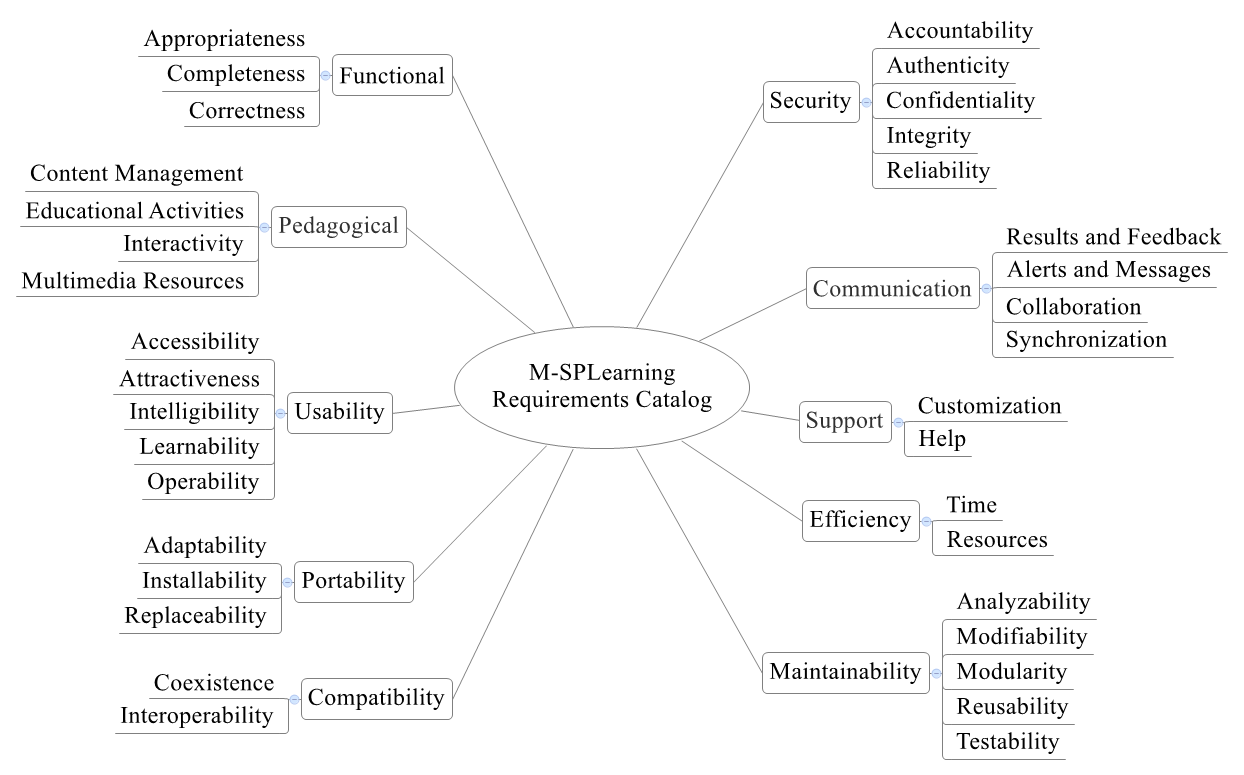
\includegraphics[scale=0.3815]{figures/section3/MSPLCatalog}
    \caption{M-SPLearning Requirements Catalog \cite{falvojr14b}.}
    \label{figureMSPLCatalog}
\end{figure}

%Com base no catálogo de referencia, observou-se que a maioria dos requisitos originalmente propostos eram equivalentes, direta ou indiretamente, às características e subcaracterísticas da norma ISO/IEC 25010. Com isso, acredita-se que a derivação do catálogo forneceu os requisitos educacionais móveis necessários para a concepção da LPS deste trabalho.
Based on the reference catalog, we could observe that most of the requirements originally proposed was equivalent, directly or indirectly, to the characteristics and subcharacteristics of ISO/IEC 25010. %Thus, it is believed that the performed  derivation provided us the educational requirements necessary for the M-SPLearning.
%Em termos estruturais, o catálogo resultante apresentou 10 requisitos primários e 35 secundários. Por exemplo, o elemento Support apresenta características comuns como a internacionalização de mensagens (provida pelo requisito Customization) e ajuda em dúvidas frequentes (Help).
In structural terms, the resulting catalog has 10 primary and 35 secondary requirements. For example, the \textit{Support} element has common features such as internationalization of messages (provided by \textit{Customization} requirement) and helps to frequently asked questions (\textit{Help}).

%Apesar de possuir requisitos genéricos e aplicáveis a outros domínios, o catálogo proposto também possui características específicas para aplicações m-learning. Por exemplo, a maior parte dos requisitos derivados a partir de Pedagogical e Communication representam necessidades essenciais ao domínio educacional móvel.
Despite having generic requirements, the proposed catalog also has specific features for m-learning applications. For instance, most of the requirements derived from \textit{Pedagogical} and \textit{Communication} represent essential requirements to the mobile educational domain.

%Em termos pedagógicos, o gerenciamento de conteúdos educativos é fundamental para o desenvolvimento das atividades educacionais. Além disso, a presença de recursos multimédia pode proporcionar acesso a informação de uma forma mais atrativa. Tais peculiaridades sintetizam os requisitos classificados pelo item Pedagogical.
In pedagogical terms, the educational content management is essential for the development of educational activities. Furthermore, the presence of multimedia resources can provide access to information in a more attractive way. Such peculiarities summarize the requirements classified by the \textit{Pedagogical} item.

%Por sua vez, os requisitos provenientes de Comunucation representam funcionalidades relacionadas à troca de mensagens, alertas e o compartilhamento de resultados ou feedbacks, tornando o aprendizado, mais colaborativo e dinâmico. Outra característica importante é a sincronização dos dados de uma aplicação m-learning, pois os usuários podem possuir e utilizar mais de um dispositivo móvel ou plataforma. 
The requirements from \textit{Communication}, in turn, represent features related to the exchange of messages, alerts and sharing results or feedback, making the learning more collaborative and dynamic. Another important feature is the synchronization of data from a mobile learning application since users can have more than one mobile device or platform.

%A fim de avaliar o catálogo de requisitos proposto para a M-SPLearning uma validação adicional actividade foi conduzida. Neste sentido, um formulário on-line foi preparado a fim de verificar informalmente as principais questões técnicas relacionadas ao catálogo. O formulário foi disponibilizado em uma estrutura de checklist, com o objetivo de mensurar a opinião de especialistas na área de engenharia de software.
To evaluate the requirements catalog proposed for the M-SPLearning, an additional validation activity was conducted. An online form was prepared in order to informally check the main technical issues related to the catalog. The form was structured as a checklist, with the aim to measure the opinions of specialists in software engineering area.

%O documento contou com 12 questões de múltipla escolha, onde as duas primeiras eram relacionadas à experiência dos participantes nos conceitos de LPS e m-learning. Nesse caso, as opções possíveis foram: Proficiente, Intermediário e Novato. As dez  questões restantes referiam-se ao catálogo de requisitos da M-SPLearning, por exemplo: O catálogo compreende requisitos adequados ao domínio?. Para essas perguntas as opções: Adequado, Regular e Insatisfatório foram aplicadas.
The checklist was composed of 12 multiple choice questions, where the first two questions were related to the background of the participants on SPL and m-learning concepts. In this case, the possible options were ``Expert", ``Intermediate" and ``Novice". The ten remaining questions were related to the M-SPLearning requirements catalog, such as: \textit{``The catalog comprises appropriate requirements to the domain?"}. To these questions the options ``Adequate", ``Regular" and ``Unsatisfactory" were applied.

%Para aplicação do formulário online alguns grupos de pesquisa foram notificados via e-mail com um convite para a participação voluntária no checklist. Após alguns dias o formulário foi finalizado com um total de 11 participantes.
%To apply the online form several research groups were notified via email with an invitation for voluntary participation in the checklist. After a few days the form was completed with a total of eleven participants.

%Os resultados coletados mostraram que, na visão dos participantes, o catálogo de requisitos está adequado ou regular a todos os itens avaliados. Além disso, nenhuma das questões relacionadas ao catálogo de requisitos da M-SPLearning foi respondida como insatisfatória. A Tabela \ref{tableMSPLChecklist} sintetiza as avaliações médias obtidas a partir dos 11 formulários de ckecklist submetidos.
The questionnaire was answered by 11 participants and the results showed that the requirements catalog was ``Adequate", with a mean of 60.90\%, and was ``Regular", with a mean of 39.10\%, in all evaluated items. Furthermore, none of the questions related to the requirements catalog of the M-SPLearning was answered as ``Unsatisfactory". 

%Table \ref{tableMSPLChecklist} summarizes the average ratings obtained from submitted forms.
%
%\begin{table}
%    \caption{M-SPLearning Requirements Catalog Checklist Summary.}
%    \centering
%    \scriptsize
%    \begin{tabular}{cc}
%        \toprule
%        \textbf{Option} & \textbf{Average Percentage Obtained} \\
%        \midrule
%        Adequate       & 60.90\% \\
%        Regular        & 39.10\% \\
%        Unsatisfactory & 0.00\% \\
%        \bottomrule
%    \end{tabular}
%    \label{tableMSPLChecklist}
%\end{table}
%
%A sumarização dos resultados foi considerada uma validação preliminar, visto que o preenchimento de um checklist anônimo não caracteriza uma técnica de validação formal. Desta forma, o checklist proposto consistiu em uma validação inicial que deve ser complementada com novas técnicas no futuro. Todavia, esta atividade de validação foi importante para avaliar o artefato que sintetizou os requisitos elicitados para a M-SPLearning.
%The summary of the results was considered a preliminary validation, since the completion of an anonymous checklist does not characterize a formal validation technique. Therefore, the proposed checklist consisted of an initial validation that should be supplemented with new techniques in the future. However, this validation activity was important to evaluate the asset that summarized the elicited requirements for the M-SPLearning.
Although preliminary, the informal validation performed was important to evaluate the set of requirements elicited for M-SPLearning.

%A próxima etapa da atividade de Análise de Domínio consiste em identificar as variabilidades existentes nos produtos da M-SPLearning, de acordo com a definição da abordagem proativa. Nesse sentido, as variabilidades representam a forma pela qual os produtos são diferenciados em uma LPS, tornando possível a geração dos produtos específicos suportados pela LPS. Em termos práticos, as variabilidades geralmente são identificadas e representadas através do conceito de features.
The next stage of the Domain Analysis activity was the identification of the existing variabilities in the M-SPLearning products \cite{krueger02}. In this sense, variabilities represent the way in which products are differentiated in an SPL, making possible the generation of specific products supported by the SPL \cite{vangurp01}. In practical terms, variabilities are generally identified and represented through the features concept \cite{bosch01, kang90}.

%No contexto da M-SPLearning, o catálogo de requisitos foi analisado, e suas características serviram como base para a criação de um modelo feature em conformidade aos requisitos elicitados (Figura X). A interpretação do modelo de features é simples e segue os conceitos tradicionais idealizados pela abordagem Feature-Oriented Domain Analysis (FODA). Basicamente, cada requisito concreto presente no catálogo M-SPLearning foi transformado em uma feature primária. Com isso, foram modeladas 16 features obrigatórias e 14 features opcionais.
In the context of M-SPLearning, the requirements catalog was analyzed and their characteristics were used as the basis for creating a feature model with compliance to the requirements elicited (Figure \ref{figureMSPLFeatureModel}). The interpretation of the feature model is straightforward and follows the traditional concepts conceived by the Feature-Oriented Domain Analysis approach (FODA) \cite{kang90}. Basically, each concrete requirement in M-SPLearning catalog was mapped to a primary feature. Thus, 16 mandatory features and 14 optional features were modeled.



%Com relação ao catálogo, alguns dos requisitos elicitados foram considerados muito abstratos ou onipresentes em relação do domínio m-learning e, por isso, não foram transformados em features, são eles: (i) Functional; (ii) Portability; (iii) Efficiency; e (iv) Maintainability. Por outro lado, as features primárias e suas respectivas responsabilidades no domínio das aplicações m-learning são apresentadas a seguir, sintetizando as contribuições relacionadas à Análise de Domínio:
With regard to the catalog, some of the elicited requirements were considered too abstract or ubiquitous over the m-learning domain and, therefore, they were not mapped to features (\textit{Functional}, \textit{Portability}, \textit{Efficiency}, \textit{Maintainability}). The primary features and their responsibilities for m-learning applications are the following:

\begin{itemize}

    %Incorpora requisitos educacionais e pedagógicos, provendo as principais características presentes em aplicações m-learning para atividades de ensino e treinamento. A subfeature Interactivity é opcional, uma vez que está relacionada a interatividade por meio de redes sociais. As subfeatures Content Management, Educational Activities e Multimedia Resources são obrigatórias, onde a última delas possibilita a escolha de um ou mais recursos multimédia como apoio ao ensino.
    \item \textit{Pedagogical}: incorporates educational and pedagogical requirements, providing the main characteristics of m-learning applications for teaching and training activities. The subfeature \textit{Interactivity} is optional, as it is related to interactivity through social networks. The subfeatures \textit{Content Management}, \textit{Educational Activities} and \textit{Multimedia Resources} are mandatories; in the latter offers a choice of one or more multimedia resources to support teaching.
    
    %Apresenta características essenciais no que diz respeito à interface visual de uma aplicação m-learning. Tais características são fundamentais para a aceitação do produto no mercado. Essa feature e suas variações determinam que todos os produtos gerados pela LPS devem ter um padrão de usabilidade, provendo qualidade aos usuários finais. Com isso, todas as features em questão foram definidas como obrigatórias.
    %A plataforma Android possui diversas imposições em termos de usabilidade, com o objetivo de padronizar e maximizar a experiência de seus usuários, por este motivo as features em questão foram definidas como abstratas.
    \item \textit{Usability}: address the essential characteristics with respect to the visual interface of a mobile learning application. These characteristics are fundamental to the acceptance of the product on the market. This feature and its variations establish that all products generated by an SPL must adopt a standard of usability, providing quality to final users. Thus, all these features were defined as mandatory.


\begin{figure}[!ht]
    \centering
    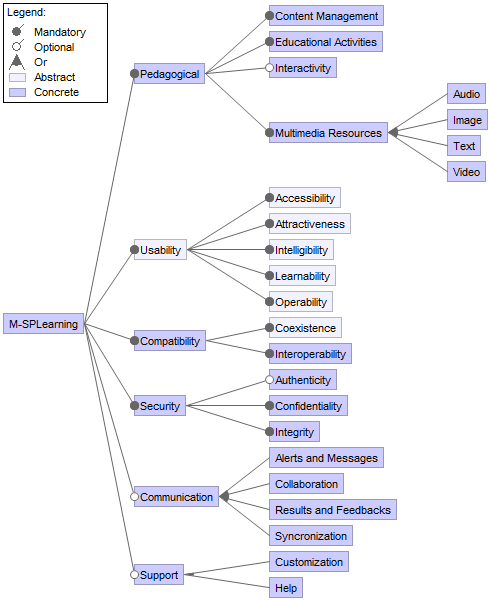
\includegraphics[scale=0.8]{figures/section3/MSPLFeatureModel}
    \caption{M-SPLearning Feature Model \cite{falvojr14a, falvojr14b}.}
    \label{figureMSPLFeatureModel}
\end{figure}

    %Engloba a coexistência e capacidade de trocar informações com outros sistemas no mesmo ambiente operacional. Por se mostrar essencial a aplicativos móveis, essas features foram definidas como obrigatórias.
    \item \textit{Compatibility}: includes the coexistence and ability to exchange information with other systems on the same operating environment. It is essential for mobile applications, thus their features were defined as mandatory.
    
    %Trata-se de uma feature fundamental para qualquer aplicativo m-learning, uma vez que existem aspectos que devem ser garantidos para que os usuários confiem no produto gerado. As features que representam a integridade e confidencialidade foram definidas como obrigatórias devido a sua importância em termos de seguraça. Já a feature Authenticity é opcional porque nem todo aplicativo m-learning possui autenticação explícita de seus usuários.
    \item \textit{Security}: this is a key feature since any mobile application should send and receive data securely. The features \textit{Integrity} and \textit{Confidentiality} were defined as mandatory due to its importance in security terms. On the other hand, the \textit{Authenticity} feature is optional because not every m-learning application has explicit authentication of its users.
    
    %Provê o transporte de informações entre os usuários do aplicativo, possibilitando a troca de mensagens, a verificação resultados de testes e até mesmo a sincronização de atividades realizadas em outros dispositivos móveis. Essa feature é opcional e suas subfetaures possuem essa mesma definição, possibilitando qualquer combinação possível entre elas.
    \item \textit{Communication}: responsible for changing information among users of the application, enabling the exchanging of messages, testing results and even synchronizing activities in other mobile devices. This feature and subfeatures are optional, allowing any possible combination among them.
    
    %Trata-se de uma feature considerada um diferencial de qualidade para os produtos em que ela está presente, pois provê alternativas de apoio ao usuário, como ajuda e internacionalização. Foi classificada como opcional por não ser um pré-requisito, assim como suas subfeatures.
    \item \textit{Support}: this feature provides some interesting alternatives to user, such as help and internationalization. It was classified as an optional because it is not a prerequisite as well as its subfeatures.
\end{itemize}

\subsubsection{Definition of Architecture}

%A partir do modelo de features apresentado anteriormente, definimos uma arquitetura de software aderente às necessidades do domínio educacional móvel. Tal arquitetura e seus respectivos componentes representam de forma abstrata os ativos centrais da M-SPLearning. Nesse sentido, a maioria das abordagens desenvolvidas para auxiliar no gerenciamento de variabilidades envolvem diversos conceitos e modelos de representação. A abordagem SMarty, em especial, é baseada na UML, amplamente aceita pela comunidade científica. Com isso, devido a sua facilidade de uso e resultados experimentalmente avaliados a SMarty foi escolhida para apoiar esta atividade da M-SPLearning.
From the feature model we defines an adherent software architecture to the mobile domain educational needs. Such an architecture and its components represent abstractly the core assets of M-SPLearning. Accordingly, most of the approaches developed to assist in the management of variability involve several concepts and representation models. SMarty, in particular, is based on UML, widely accepted by scientific and industrial communities. Thus, due to its ease of use and results (experimentally evaluated), SMarty was chosen to support the design of the M-SPLearning promising architecture.

%A abordagem SMarty foi essencial durante todo o processo de desenvolvimento da LPS proposta, sobretudo por agregar seu perfil aos modelos UML para representação das similaridades e, principalmente, das variabilidades da M-SPLearning, como é o caso do diagrama de componentes arquiteturais ilustrado na Figura \ref{figureMSPLArchitecture}. Com base no diagrama arquitetural é possível identificar a base estrutural utilizada para a construção da M-SPLearning. O pacote com os ativos centrais engloba os componentes que representam as features definidas como concretas no modelo de features.
SMarty played a important role through the development of M-SPLearning, providing the standards defined by the SMartyProfile to represent the similarities and, especially, the variabilities of M-SPLearning. The diagram of architectural components illustrated in Figure \ref{figureMSPLArchitecture} represents one of the diagrams developed with the support of the SMarty approach. Based on the architectural diagram it is possible to identify the structural basis used to the construction of the M-SPLearning. The package \textit{Core Assets} comprises concrete features as shown on Figure \ref{figureMSPLFeatureModel}.

\begin{figure}
    \centering
    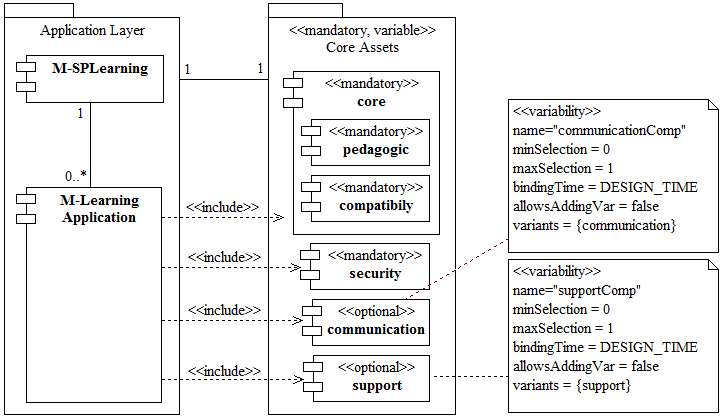
\includegraphics[scale=0.55]{figures/section3/MSPLArchitecture}
    \caption{M-SPLearning SMarty-based Architecture Diagram.}
    \label{figureMSPLArchitecture}
\end{figure}

%Os componentes que representam features específicas do domínio m-learning foram agrupados e nomeados como core. Assim, foi possível unificar os módulos fundamentais aos produtos gerados através da M-SPLearning. Além disso, é possível identificar alguns dos elementos da abordagem SMarty, que nesse caso representam as variabilidades em alto nível.
The components that represent the specific features of the m-learning domain were grouped in the package \textit{core}. Thus, it was possible to unify the fundamental modules to products generated by M-SPLearning. Furthermore, it is possible to identify some of the elements of SMarty, which in this case represent the variabilities at component level.

%A camada de aplicação, por sua vez, contém um componente que caracteriza a M-SPLearning, identificando sua associação com os ativos centrais e explicitando a possibilidade de criação de produtos, também representados como componentes. Cada produto gerado pode incluir as dependências disponíveis nos ativos centrais, fazendo com que cada produto possa utilizar dependências diferentes de acordo com as configurações definidas na M-SPLearning.
The \textit{Application Layer} contains a component that characterizes the M-SPLearning, identifying its association with core assets and making explicit the possibility of products derivation. Each product may include the components available in \textit{Core Assets}, making each m-learning application use different features according to your configurations defined in M-SPLearning.

%A próxima seção apresenta a atividade seguinte, que detalha cada um dos componentes representados como ativos centrais na M-SPLearning. O objetivo é detalhar suas similaridades e variabilidades para a definição do Plano de Produção, última atividade da Análise de Domínio.
%The next section presents the Components Project, which details each of the components represented as core assets in M-SPLearning. The goal is to detail their similarities and variabilities to define the Production Plan, last activity of Domain Analysis.

\subsubsection{Components Design}

%Esta fase deve ser conduzida para projetar as variabilidades e similaridades identificadas pela Análise de Domínio. Nesse sentido, os componentes, arquitetonicamente armazenados junto aos ativos centrais, tiveram suas respectivas \textit{features} visualmente representadas por meio de um diagrama de componentes SMarty, ilustrado na Figura \ref{fig:msplDesign}.
This phase is responsible for the designing of the variabilities and similarities identified in the Domain Analysis. Accordingly, the core assets elements were visually represented by a SMarty diagram components, shown in Figure \ref{figureMSPLDesign}.

\begin{figure}[!ht]
\centering
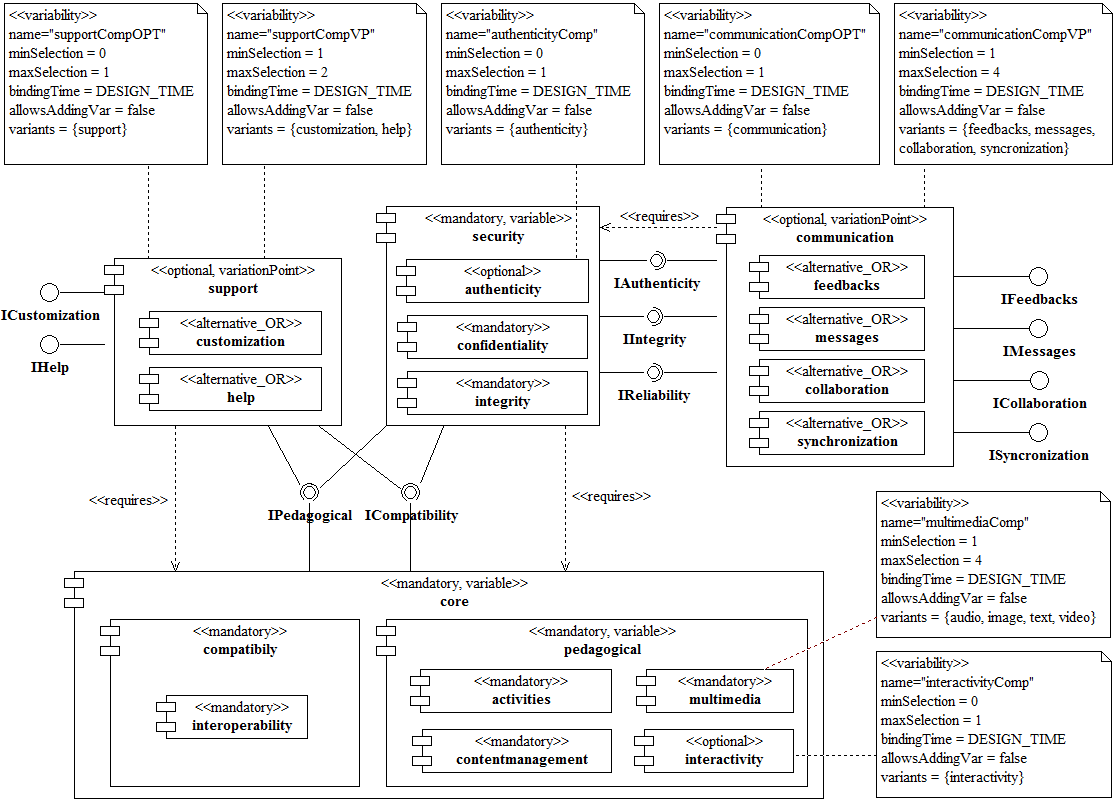
\includegraphics[scale=0.46]{figures/section3/MSPLDesign}
\caption{M-SPLearning SMarty-based Components Diagram.}
\label{figureMSPLDesign}
\end{figure}

%Por meio desse diagrama de componentes é possível visualizar todas as features concretas contempladas pela M-SPLearning. Os componentes resultantes foram rotuladas com os estereótipos característicos da abordagem SMarty. Esse diagrama permite a analise da quantidade de configurações possíveis aos aplicativos m-learning contemplados pela LPS.
Analyzing this component diagram it is possible to notice all concrete features covered by M-SPLearning. The resulting components are labeled with the characteristic stereotypes of SMarty approach. This diagram allows the analysis of the possible configurations for m-learning applications covered by the SPL.
%Por exemplo, o componente multimedia foi modelado como uma variabilidade (esteriótipo variability), ou seja, ele pode ser configurado para que uma LPS crie aplicações m-learning customizadas de acordo com suas configurações. Dessa forma, uma aplicação poderia ser configurada para possuir no mínimo um e no máximo quatro recursos multimédia (audio, image, text e video), conforme as notações "minSelection" e "maxSelection". Uma observação relevante é que qualquer componentes cujo filho foi modelado como uma variabilidade deve ser marcado como variável (esteriótipo variable).
For example, the \textit{multimedia} component was modeled with variability stereotype, ie it can be configured so that the SPL create specific m-learning applications according to your settings. Thus, a product can be configured to have among one and four \textit{multimedia} resources (audio, image, text and video), according to the notations ``minSelection" and ``maxSelection". Its important to highlight that any components formed for other components with variability should be tagged with the variable stereotype.

%Com ênfase no domínio explorado, os componentes pedagogical e communication se destacam, assim como seus requisitos. Nesse sentido, a maioria dos componentes pedagógicos são obrigatórios, com variabilidades possíveis em termos de interatividade e recursos multimídia (já explanada anteriormente). Por sua vez, os componentes agrupados em communication são alternativos, sendo que ao menos um deles deve agregar sua funcionalidade aos produtos gerados.
With emphasis on the explored domain, the \textit{pedagogical} and \textit{communication} components stand out, as well as your requirements. In this sense, most \textit{pedagogical} subcomponents are mandatories, with possible variabilities in terms of \textit{interactivity} and \textit{multimedia} features. In turn, the \textit{communication} subcomponents are alternatives, and at least one of them must provide its functionalities to the generated products.

%Também fica explícito o relacionamento de dependência entre os componentes modelados. Como definido anteriormente, o componente core unifica as features integralmente obrigatórias ao domínio m-learning, tornando-se necessário, direta ou indiretamente, aos componentes security, communication e support. A particularidade aqui fica por conta do componente communication, dependente do componente security, que por sua vez está relacionado com o componente core, fazendo com que o componente communication também tenha acesso a essa dependência. Isso garante a imposição arquitetônica de que todos os componentes parcialmente mandatórios ou opcionais dependam do componente core, que proverá as características fundamentais da M-SPLearning.
The dependency relationship between the modeled components also becomes explicit. As previously defined, the \textit{core} component unifies the mandatory features to m-learning domain, being necessary, directly or indirectly, to the \textit{security}, \textit{communication} and \textit{support} components. Particularly, the \textit{communication} component depends on the \textit{security} component, which in turn is related to the \textit{core} component. As a consequence, the \textit{communication} component also knows the \textit{core}.

%A partir do Projeto de Componentes aferidos pela LPS, torna-se possível a definição de um Plano de Produção que transforme as representações abstratas em produtos de software concretos, com suas respectivas variabilidades. A seção a seguir conclui a Análise de Domínio definida para a M-SPLearning.
Finally the Components Project, it is possible to define a Production Plan to transform the abstract representations in concrete software products, with their respective variabilities.

\subsubsection{Production Plan}

%O Plano de Produção prescreve como os produtos devem ser gerados a partir dos ativos centrais definidos para a LPS. Para isso, um diagrama de atividades usando a abordagem SMarty foi modelado, expondo as variabilidades possíveis durante o processo de criação de um produto (Figura \ref{figureMSPLProductionPlan}). Basicamente, este plano pode ser considerado um ativo central da M-SPLearning, assim como qualquer outro artefato que contribua para a criação sistemática de seus produtos. 
The Production Plan prescribes how the products should be generated from the core assets identified for the SPL. For this, an activity diagram using the SMarty approach was modeled, exposing the possible variabilities in the process of creating a product (Figure \ref{figureMSPLProductionPlan}). Basically, this plan can be considered a core asset of M-SPLearning, just like any other artifact that contributes to the systematic creation of their products.

\begin{figure}
\centering
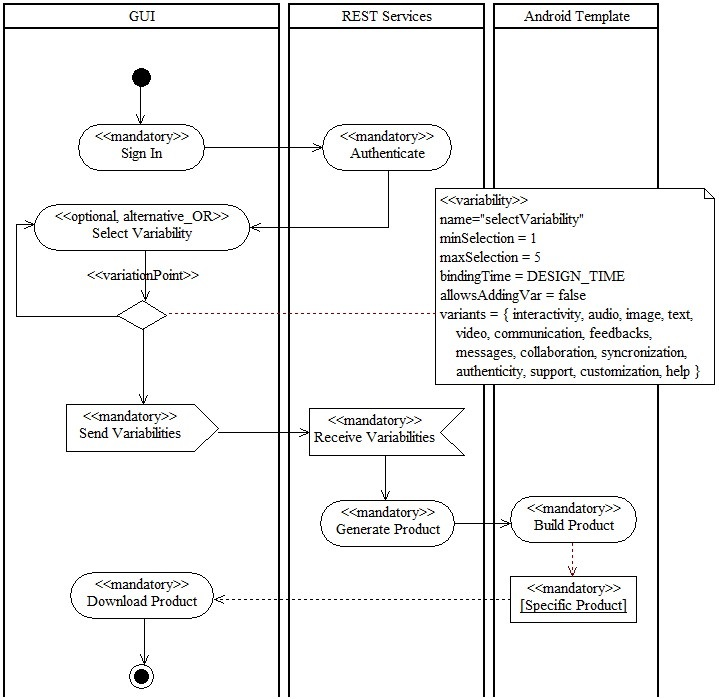
\includegraphics[scale=0.5]{figures/section3/MSPLProductionPlan}
\caption{M-SPLearning SMarty-based Production Plan.}
\label{figureMSPLProductionPlan}
\end{figure}

%O ponto de variação definido no plano de produção expõe todas as variabilidades elicitadas para a M-SPLearning. Desta forma, a customização dos produtos foi centralizada em um único ponto, agilizando o processo de configuração e geração dos aplicativos m-learning, provenientes da LPS proposta.
The variation point defined in the production plan exposes all variabilities elicited for M-SPLearning. Thus, the customization of the products was centralized at a single point, streamlining the configuration process and generation of m-learning applications by the SPL proposal.

%Cada raia do diagrama representa um módulo específico, sendo possível identificar algumas características arquiteturais da M-SPLearning. Uma das mais importantes neste sentido é a utilização do conceito de REpresentational State Tranfer (REST). Essa característica permite a criação e consumo de web services por meio do padrão Hypertext Transfer Protocol (HTTP), tornando viável a utilização de arquiteturas emergentes, como a Service-Oriented Architecture (SOA), também no contexto de aplicações móveis.
Each swimlane of the diagram represents a specific module, making it possible to identify some architectural characteristics of the M-SPLearning. One of the most important with this regard is the use of the REpresentational State Tranfer (REST) \cite{fielding00} architectural style. This concept allows the creation and consumption of web services using the Hypertext Transfer Protocol (HTTP), making possible the use of emerging software architectures such as Service-Oriented Architecture (SOA), also in the context of mobile applications.

%A seguir cada módulo representado no diagrama de atividades é sintetizado, considerando suas características técnicas e responsabilidades em termos práticos:
Next, each module represented in Figure \ref{figureMSPLProductionPlan} is synthesized considering its main characteristics in technical terms:

\begin{itemize}
    %Módulo que provê a interface gráfica dos usuários da LPS, ou seja, as representações visuais com as quais os usuários interagem para a geração dos produtos apoiados pela M-SPLearning. Neste módulo, é possível configurar as variabilidades e visualizar as similaridades, além de solicitar a geração de um produto personalizado. Este módulo foi implementado utilizando apenas tecnologias client-side, em especial HTML, JavaScript e CSS. A ideia foi demonstrar a interoperabilidade em uma arquitetura SOA, já que foram implementados todos os serviços usando REST, conforme o item a seguir.
	\item \textbf{\textit{Graphical User Interface (GUI):}} module responsible for providing the visual representations with which users interact to generate the products supported by M-SPLearning. In this module, the variabilities can be configured, allowing the generation of a customized product. This module was implemented using only client-side technologies, especially HTML, JavaScript and CSS. The idea was to demonstrate interoperability in a SOA architecture, since all services were implemented using REST.
	
	%Módulo desenvolvido a partir da abstração arquitetônica REST, que se caracteriza pelo uso de tecnologias e protocolos da web para a criação e entrega de serviços. Este estilo é totalmente aderente ao padrão arquitetural SOA e assegura a disponibilidade e consumo de web services de uma forma simples e eficiente. Este módulo corresponde à principal interface entre os produtos gerados pela M-SPLearning e suas features. Ele acessa um banco de dados remoto, onde todas as informações são armazenadas, incluindo as features (similaridades e variabilidades) especificadas via GUI. A centralização dos dados no módulo de serviços torna-o essencial para os outros (GUI e Android Template), uma vez que ambos consomem os web services disponibilizados por ele.
	\item \textbf{\textit{REST Services:}} module developed from the REST architectural abstraction, which is characterized by the use of technologies and protocols of the web for the creation and delivery of services. This style is fully adherent to the SOA architectural pattern and ensures the availability and consumption of web services in a simple and efficient way. This module is the main interface between the products generated by the M-SPLearning and its features. It accesses a remote database where all the information is stored, including features (similarities and variabilities) configured from the \textit{GUI}. The centralization of data in the \textit{REST Services} module is essential for other (\textit{GUI} and \textit{Android Template}), since both consume the web services provided by it.
	
	%Este módulo provê um template genérico para a customização dos produtos. Isso permite que um serviço, disponível no módulo REST Services, execute uma compilação personalizada de acordo com as variabilidades configurados no módulo GUI. O resultado é um Android Application Package (APK) com todas as features pré-configuradas, o que permite a instalação do produto customizado em qualquer dispositivo Android.
	\item \textbf{\textit{Android Template:}} module responsible for providing a generic template for the customization of products. This allows a service, available in \textit{REST Services} module, execute a custom build according to the variabilities configured in the \textit{GUI}. The result is an Android Application Package (APK) with all pre-configured features, allowing the installation of custom product on any Android device.
\end{itemize}

%Considerando a necessidade de construção de aplicações m-learning com maior qualidade e reúso, os esforços para o desenvolvimento de LPS que lidam com aspectos SOA ganharam especial importância no contexto móvel. A adoção de uma abordagem SOA torna-se cada vez mais relevante, principalmente porque torna mais fácil e flexível a construção de suas aplicações, promovendo interoperabilidade e reutilização, o que corrobora com as definições arquiteturais propostas no plano de produção.
Considering the need of building m-learning applications with higher quality and reuse, efforts for the development of SPL dealing with SOA aspects gained special importance in the mobile context \cite{marinho10, nascimento11}. The adoption of an SOA approach becomes increasingly important, especially because it makes easy and flexible to build their applications, promoting interoperability and reuse, which agrees with the architectural definitions proposed in the production plan.

%A M-SPLearning foi elaborada a partir de um processo baseado em práticas e conceitos relevantes no âmbito da Engenharia de Software. Com isso, a M-SPLearning utilizou um processo sequencial para sua definição, abordando as dificuldades da análise de elementos do domínio e as definições arquiteturais necessárias para sua implementação proativa. A próxima seção trata da atividade primária subsequente, a Engenharia de Aplicação.
M-SPLearning was elaborated from a process based on relevant practices and concepts in software engineering. Thus, M-SPLearning has used an incremental process for its definition, addressing the difficulties of domain analysis and the necessary architectural definitions for a proactive implementation. The next section deals with the subsequent SPL activity, the AE.

\subsection{Application Engineering}\label{section32}

%Esta atividade depende essencialmente dos artefatos de saída da Engenharia de Domínio, que agora atuam como artefatos de entrada. A partir dos ativos gerados, um conjunto específico de features foi selecionado para a implementação da M-SPLearning. Essa redução de escopo foi definida com o objetivo de viabilizar a avaliação experimental da M-SPLearning. Dessa forma, com um número reduzido de features, foi possível implementar e avaliar a LPS em um prazo aceitável.
This activity depends on the output artifacts of DE, which now act as input devices. Using these artifacts, a specific set of features was selected for the implementation of M-SPLearning. This reduction in scope was defined in order to enable the experimental evaluation of the M-SPLearning. Thus, with a limited number of features, it was possible to implement the SPL in 188 hours, enabling even their experimental evaluation.

%No contexto deste trabalho, as features relacionadas às atividades pedagógicas e de segurança foram priorizadas e implementadas. O motivo dessa escolha é que as features em questão representam os requisitos funcionais mínimos de uma aplicação m-learning, são eles: (i) Pedagogical: inclui a realização de atividades educacionais através do gerenciamento de conteúdos interativos e recursos multimédia; (ii) Security: agrega em termos de confidencialidade e integridade dos dados, além da possibilidade de autenticação dos usuários; e (iii) Communication: incluiu apenas a feature relacionada à sincronização de dados.
In the context of this work, the features related to teaching and security activities were prioritized and implemented. The reason for this choice is that such features are the minimum functional requirements of a m-learning application: (i) \textit{Pedagogical}: includes conducting educational activities through the management of interactive and multimedia content; (ii) \textit{Security}: provides confidentiality and integrity of data, added by the ability to authenticate users; and (iii) \textit{Communication}: includes the feature related to data synchronization.

%Tecnicamente, a M-SPLearning apresenta a visão lógica de uma LPS definida para configuração e geração de aplicações m-learning na plataforma Android. Sua implementação foi feita predominantemente em Java e seu código fonte pode ser consultado a partir do repositório open source GitHub.
In technical terms,  M-SPLearning presents the logical view of an SPL defined for configuration and generation of m-learning applications on the Android platform. Its implementation was made predominantly in Java and its source code is available\footnote{http://github.com/falvojr/msplearning} on GitHub open source repository.

%Por definição, a Engenharia de Aplicação instancia os ativos centrais de uma LPS para geração de produtos específicos. Para isso, o plano de produção, até então abstrato, foi utilizado para a construção de seus respectivos módulos concretos. No contexto desta atividade, o módulo GUI foi inevitavelmente o mais explorado, porque todos os produtos são gerados através dele.
By definition, the AE instantiates the core assets of SPL to generate specific products. For this, the production plan was used to build the respective concrete modules. In the context of this activity, the \textit{GUI} module is inevitably the most exploited, because all products are generated therethrough.

%A primeira interação entre usuário e a M-SPLearning ocorre em uma página inicial web. Nela, os usuários podem registrar-se e, posteriormente, autenticar-se na aplicação. Essa interface visual também introduz o domínio e os principais objetivos da M-SPLearning, contextualizando seus usuários. Outro aspecto relevante foi a construção de suas páginas web completamente baseadas no conceito de layouts responsivos, o que, dentre outras tendências, tornou a representação visual da LPS ainda mais dinâmica e flexível. A Figura \ref{figureMSPLWebLogin} expõe tais características.
The first interaction between the user and M-SPLearning occurs in a web home page. Therein, users can sign up and then log into the application. This interface also introduces the domain and the main objectives of M-SPLearning. Another important aspect refers the construction of the web pages completely based on the concept of responsive layouts, which makes the visual representation of SPL even more dynamic and flexible. 

%Figure \ref{figureMSPLWebLogin} presents such characteristics.
%
%\begin{figure}
%\centering
%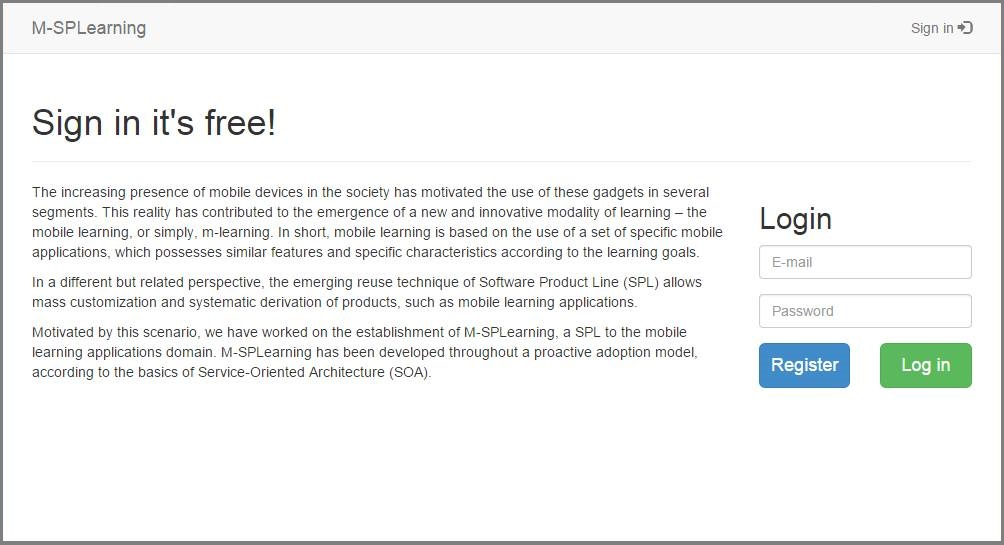
\includegraphics[scale=0.4]{figures/section3/MSPLWebLogin}
%\caption{M-SPLearning GUI Login.}
%\label{figureMSPLWebLogin}
%\end{figure}

%Com um usuário devidamente autenticado, a interface resultante é a caracterização mais evidente da M-SPLearning, já que possibilita o gerenciamento visual das variabilidades disponibilizadas pela LPS. Neste ponto, o usuário, por exemplo um professor, simplesmente realiza alguns cliques para geração de um produto específico, criando, assim, um APK com uma aplicação m-learning instalável em qualquer dispositivo Android.
With an authenticated user, the resulting interface is the most evident characterization of M-SPLearning, as it enables the visual management of variabilities provided by SPL. At this point, the user, for example a teacher, simply performs a few clicks to generate a specific product, which creates an APK that encapsulates a custom m-learning application for any Android device. The page for performing this procedure is illustrated in Figure \ref{figureMSPLWebGeneration}, which also shows the visual interface for managing the products generated by M-SPLearning. Furthermore, it is important to note that the variabilities related to features prioritized during this implementation can be configured in the products generation.

%A página para a realização desse procedimento é ilustrado pela Figura 1, que também apresenta a interface visual para o gerenciamento dos produtos gerados através da M-SPLearning. Além disso, é importante observar que as variabilidades relacionadas às features priorizadas durante essa implementação podem ser configuradas na geração dos produtos.

\begin{figure}[!ht]
\centering
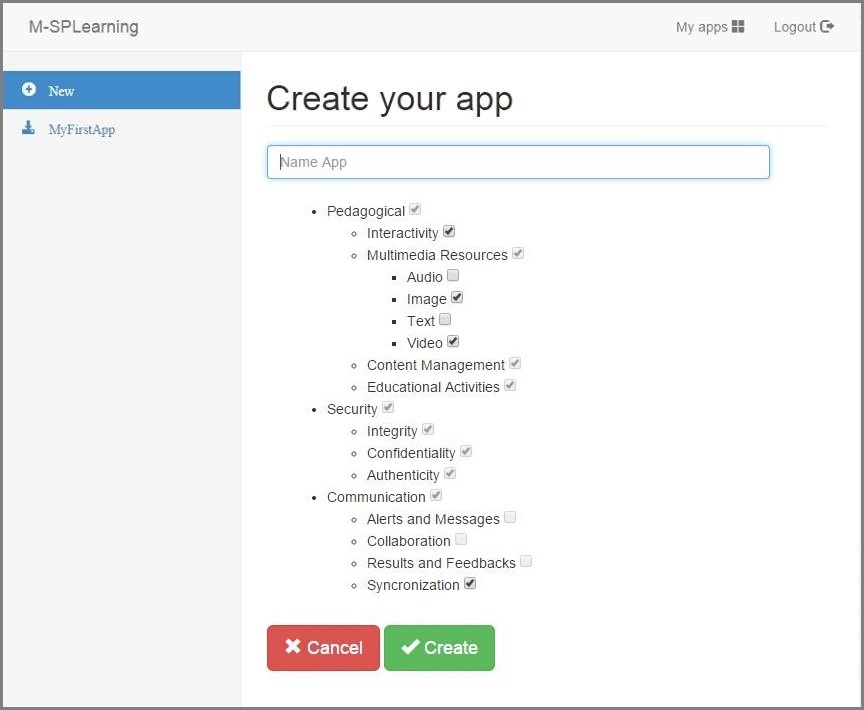
\includegraphics[scale=0.45]{figures/section3/MSPLWebGeneration}
\caption{M-SPLearning GUI Product Generation.}
\label{figureMSPLWebGeneration}
\end{figure}

%Ao solicitar a geração de um APK, os módulos REST Service e Android Template são acionados simultaneamente. Essa integração resulta na criação de um produto aderente às variabilidades selecionadas pelo usuário. A partir deste momento a aplicação m-learning gerada pode ser instalada no dispositivo móvel de qualquer professor ou aluno, que deve se registrar na aplicação móvel, caso a feature Authentication tenha sido selecionada durante a criação do APK.
When request the generation of a APK the \textit{REST Services} and \textit{Android Template} modules are triggered simultaneously. This integration results in the creation of a adherent product to user selected variabilities. Thus, the m-learning application generated can be installed on the Android device of any teacher or student, who must register with the mobile application if the feature \textit{Authentication} has been selected when creating the APK.

%A Figura 1 mostra dois produtos gerados com as variabilidades Authenticity e Interactivity configuradas de formas diferentes, nas quais: (a) o produto foi configurado apenas com a feature Authenticity; e (b) o produto foi gerado com ambas as variabilidades, o que explica o formulário de autenticação com a possibilidade de interação com algumas redes sociais.
Figure \ref{figureMSPLLogin} illustrates two products generated with \textit{Authenticity} and \textit{Interactivity} variabilities configured in different ways: (a) the product was configured with only the Authenticity feature; and (b) the product was generated with both variabilities, which explains the authentication form with the possibility of interaction with some social networking.

\begin{figure}[!ht]
\centering
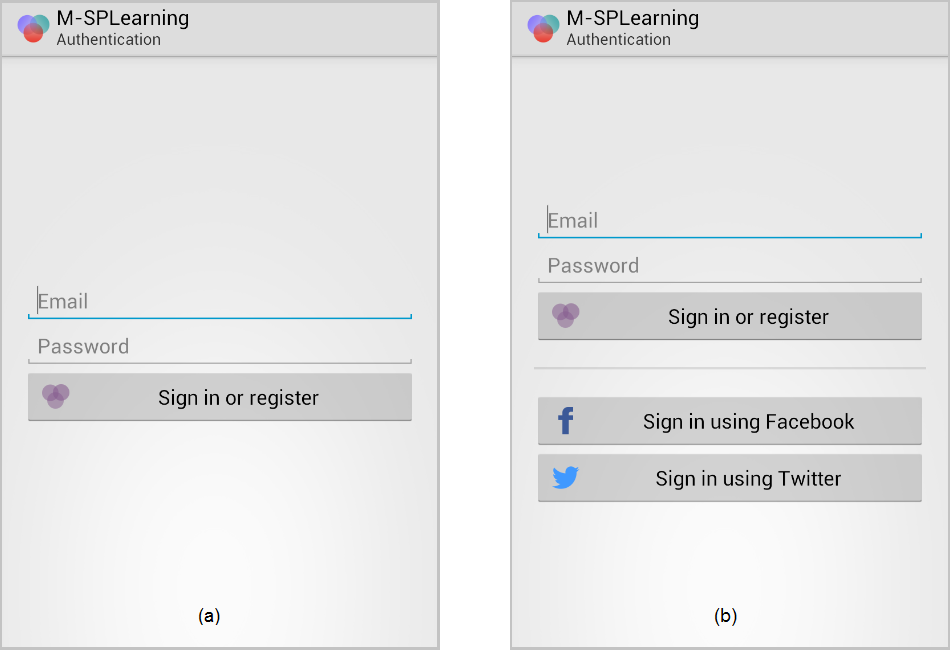
\includegraphics[scale=0.35]{figures/section3/MSPLLogin}
\caption{M-SPLearning Product Login -- Configurations of the features:\newline(a) \textit{Authenticity}; and (b) \textit{Authenticity} and \textit{Interactivity}.}
\label{figureMSPLLogin}
\end{figure}

%Observando a Figura 1 nota-se que o botão comum aos produtos também prevê a possibilidade de registro de um novo usuário. Para isso, o usuário deve apenas preencher seu e-mail e senha nos campos disponíveis para que a aplicação m-learning verifique a existência de seu usuário. Em caso negativo, o formulário de cadastro é exibido já com as informações digitadas preenchidas (Figura 2).
According to Figure \ref{figureMSPLLogin}, the common button to products also provides the possibility of registering a new user. To do this, one should fill his/her email and password in the fields available for the application to verify if the user exists (Figure \ref{figureMSPLRegister} (a)). If not, the registration form is displayed with the information previously typed (Figure \ref{figureMSPLRegister} (b)).

\begin{figure}[!ht]
\centering
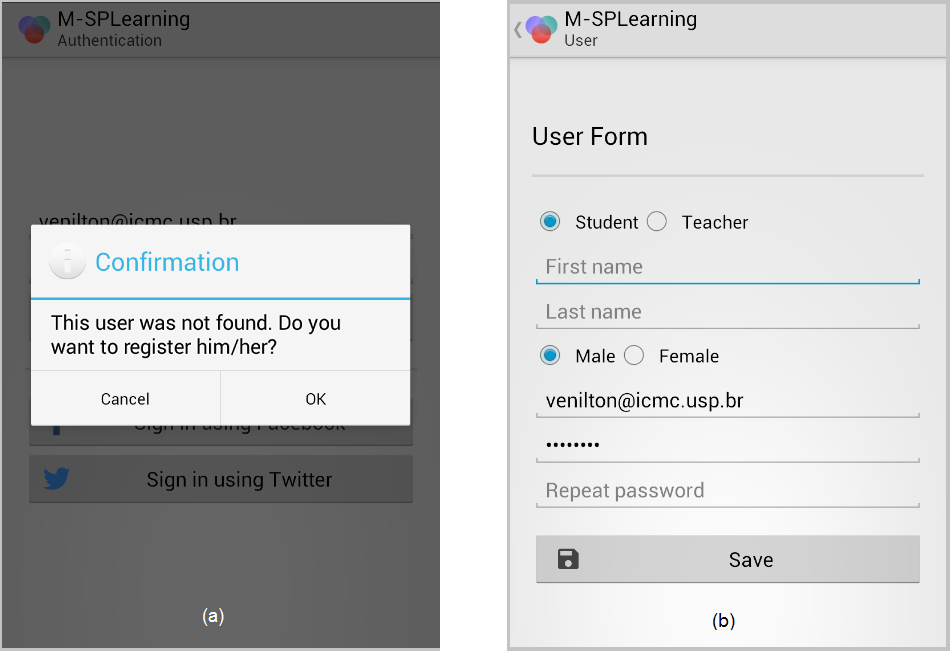
\includegraphics[scale=0.35]{figures/section3/MSPLRegister}
\caption{M-SPLearning Product Registration -- Steps for user registration:\newline(a) Confirmation message; and (b) Registration Form.}
\label{figureMSPLRegister}
\vspace{0.65cm}
\end{figure}

%O formulário de cadastro de usuário permite a seleção do tipo de acesso: professor ou aluno. Por motivos de segurança, todos os usuários registrados devem ser aprovados pelo usuário que gerou o APK. Para isso, no momento de criação da aplicação o usuário é associado a mesma com perfil administrativo. Esse aspecto deixa evidente a feature "Content Management", uma vez que cada perfil de usuário prevê acessos específicos e bem definidos. A Figura 1 ilustra um cenário possível, em que: (a) apresenta a visão de um professor; e (b) apresenta a visão de um aluno, com o adendo de que neste exemplo nenhum conteúdo educacional foi incluído, tendo em vista que o acesso a esta funcionalidade está desabilitado.
The user registration form allows the selection of the type of access: teacher or student. For security reasons, all registered users must be approved by the user who generated the APK. For this, at the time of creation of the APK the user is associated with administrative profile. This aspect makes clear the feature \textit{Content Management}, since each user profile provides specific and well-defined accesses. Figure \ref{figureMSPLDashboardApp} illustrates a possible scenario presenting: (a) the teacher's views; and (b) the student's view, but with no content, since the access to this feature is disabled.

\begin{figure}[!ht]
\centering
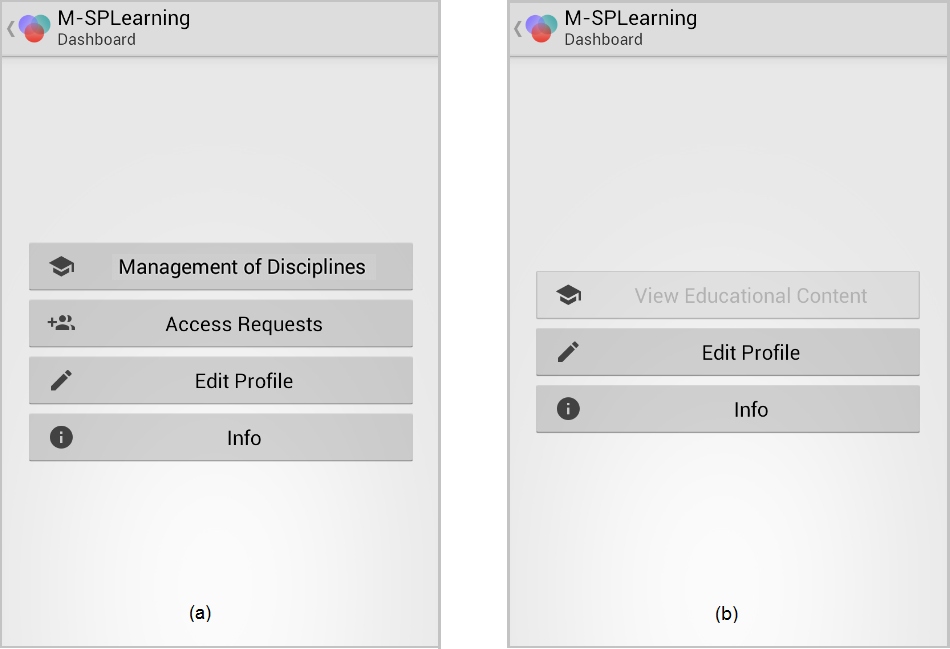
\includegraphics[scale=0.35]{figures/section3/MSPLDashboardApp}
\caption{M-SPLearning Product Dashboard -- Access Profiles:\newline(a) Teacher; and (b) Student.}
\label{figureMSPLDashboardApp}
\end{figure}

%Com um usuário devidamente autenticado e com suas respectivas funcionalidades fornecidas, a aplicação m-learning está pronta para armazenamento e compartilhamento do seu principal ativo, os conteúdos educacionais. Neste sentido, o professor pode cadastrar suas disciplinas, lições e finalmente o conteúdo de cada uma delas. Essas funcionalidades representam um contexto de uso das features Educational Activities e Multimedia Resources, também representadas pela Figura 1.
With user properly authenticated, the m-learning application is ready for storage and sharing of its main asset, the educational content. In this sense, the teacher can register his/her courses, lessons and finally the content of each lesson. These functionalities are an usage sample of the \textit{Educational Activities} and \textit{Multimedia Resources}, as shown in Figure \ref{figureMSPLEducationalContent}.

\begin{figure}[!ht]
\centering
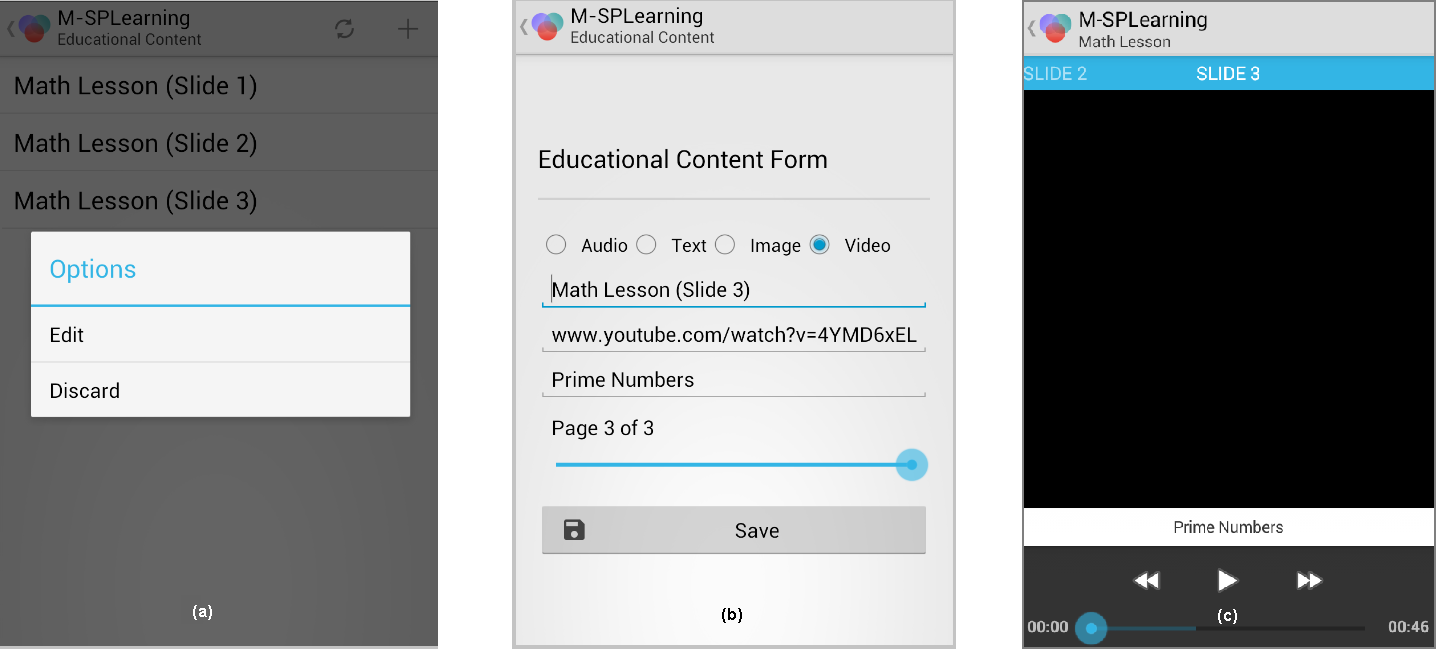
\includegraphics[scale=0.35]{figures/section3/MSPLEducationalContent}
\caption{M-SPLearning Product Educational Content Management -- Edition of educational content:\newline(a) Listing of educational content and context menu; (b) Editing form; and (c) Displaying video content.}
\label{figureMSPLEducationalContent}
\end{figure}

%De acordo com as features disponibilizadas pela M-SPLearning, nota-se a possibilidade de inclusão de conteúdos educacionais dos seguintes tipos: áudio, texto, imagem e vídeo. No exemplo apresentado, a opção de vídeo está selecionada, o que provê ao professor a inclusão de uma URL para a disponibilização do vídeo desejado aos alunos que compartilham essa aplicação.
According to the features provided by M-SPLearning, it is possible to include content of the following types: audio, text, image and video. %In the example shown, the video is selected, providing to the teacher the inclusion of an URL to the availability of the desired video students to share this application.
%Assim, os alunos visualizam os conteúdos educacionais incluídos pelos professores cadastrados na aplicação, obtendo assim acesso centralizado a sua gama de conteúdos educacionais. A Figura 1 ilustra, na perspectiva de aluno, um exemplo de conteúdo educacional do tipo vídeo.
The Figure \ref{figureMSPLEducationalContent} (c) illustrates an example of a video feature in the student perspective.

%É importante observar que foi possível incluir os requisitos previamente definidos para a construção de uma LPS. A concepção da M-SPLearning envolveu desde a análise e projeto até a implementação funcional da proposta desta pesquisa. A avaliação formal da M-SPLearning, junto de sua abordagem e principais resultados, são descritos na Seção \ref{section4}.
It is important to note that it was possible to include the requirements previously set for the construction of an SPL. The design of the M-SPLearning involved from analysis and design to functional implementation. A formal evaluation of the M-SPLearning, along with this approach and main results is described in Section \ref{section4}.